%%%%%%%%%%%%%%%%%%%%%%%%%%%%%%%%%%%%%%%%%%%%%%%%%%%%%%%%%%%%%%%%%%
%%%%%%%%%%                                              %%%%%%%%%%
%%%%%%%%%%  You can reuse this work under:              %%%%%%%%%%
%%%%%%%%%%  CC-BY-4.0 OR  etalab-2.0                    %%%%%%%%%%
%%%%%%%%%%                                              %%%%%%%%%%
%%%%%%%%%%  Henri Bretel, Robin Millman, Romain Thomas  %%%%%%%%%%
%%%%%%%%%%  2025                                        %%%%%%%%%%
%%%%%%%%%%                                              %%%%%%%%%%
%%%%%%%%%%  science.ouverte@universite-paris-saclay.fr  %%%%%%%%%%
%%%%%%%%%%  DiBISO - Université Paris-Saclay            %%%%%%%%%%
%%%%%%%%%%                                              %%%%%%%%%%
%%%%%%%%%%%%%%%%%%%%%%%%%%%%%%%%%%%%%%%%%%%%%%%%%%%%%%%%%%%%%%%%%%


%% needed for the template to find the class dir when the class folder
%% is not stored in the same directory than the main tex file
%\def\classdir{dibiso}

\newcommand{\reportyear}{2024}
\newcommand{\halcollectionid}{UNIV-PARIS-SACLAY}
\newcommand{\labacronym}{UPSaclay}
\newcommand{\labfullname}{Université Paris-Saclay}
\newcommand{\datafetchdate}{24/09/2025}
\newcommand{\watermarktext}{}

\newcommand{\anrprojectsinfo}{Le nombre d'entités affichées a été limité à 20. Dans l'API, 1637 entités ont été trouvées.\\}
\newcommand{\chaptersinfo}{}
\newcommand{\collaborationsnb}{2957}
\newcommand{\institutionsnb}{1269}
\newcommand{\countriesnb}{82}
\newcommand{\collaborationmapworldinfo}{\emoji{warning} Le traitement des données a été limité par le nombre maximal d'entités téléchargeables (1000). Des données peuvent être manquantes ou les valeurs peuvent être inférieures aux valeurs réelles. \\}
\newcommand{\collaborationmapeuropeinfo}{\emoji{warning} Le traitement des données a été limité par le nombre maximal d'entités téléchargeables (1000). Des données peuvent être manquantes ou les valeurs peuvent être inférieures aux valeurs réelles. \\}
\newcommand{\collaborationnamesinfo}{Le nombre d'entités affichées a été limité à 40. Dans l'API, 14322 entités ont été trouvées.\\}
\newcommand{\conferencesinfo}{Le nombre d'entités affichées a été limité à 40. Dans l'API, 2609 entités ont été trouvées.\\}
\newcommand{\europeanprojectsinfo}{Le nombre d'entités affichées a été limité à 20. Dans l'API, 551 entités ont été trouvées.\\}
\newcommand{\bsojournalsnbworks}{1000}
\newcommand{\bsojournalsnbworksfoundinbso}{792}
\newcommand{\bsojournalsnbjournals}{503}
\newcommand{\bsojournalsbsoversion}{2024Q4}
\newcommand{\journalsinfo}{\emoji{warning} Le traitement des données a été limité par le nombre maximal d'entités téléchargeables (1000). Des données peuvent être manquantes ou les valeurs peuvent être inférieures aux valeurs réelles. \\}
\newcommand{\journalshalinfo}{Le nombre d'entités affichées a été limité à 40. Dans l'API, 3407 entités ont été trouvées.\\}
\newcommand{\oaworksperiod}{2020 - 2024}
\newcommand{\openaccessworksinfo}{}
\newcommand{\privatesectorcollaborationsinfo}{\emoji{warning} Le traitement des données a été limité par le nombre maximal d'entités téléchargeables (1000). Des données peuvent être manquantes ou les valeurs peuvent être inférieures aux valeurs réelles. \\}
\newcommand{\workstypeinfo}{}



\documentclass[french, 11pt]{dibiso/pubpart}

\title{Publications \\ \& \\ Partenariats}

% not used
%\author{}

\date{\reportyear}

\subtitle{\textbf{\entitiesacronym} \\
  \medskip
  \entitiesfullname
}

%\titledescription{}

% Écriver votre nom entre les crochets ci-dessous, par exemple :
% \reporter{Prénom Nom}
\reporter{}
% Écriver votre adresse email entre les crochets ci-dessous, par exemple : 
% \reporteremail{reporter.email@example.com}
\reporteremail{}


%%%%%%%%%%%%%%%%%%%%%%%%%% COMMENT REMPLIR LE RAPPORT %%%%%%%%%%%%%%%%%%%%%%%%%
%                                                                             %
% Commenter des parties à exclure :                                           %
% Pour commenter des sections que vous ne souhaitez pas inclure dans le       %
% rapport final, vous pouvez utiliser le symbole % au début de chaque ligne   %
% que vous souhaitez exclure. Cela peut vous servir à ne pas afficher des     %
% sections du rapports que vous ne jugez pas appropriées pour le rapport.     %
%                                                                             %
%                                                                             %
% Créer une liste à puces :                                                   %
% Pour créer une liste à puces, utilisez l'environnement itemize. Voici un    %
% exemple :                                                                   %
% \begin{itemize}                                                             %
%     \item Premier élément de la liste                                       %
%     \item Deuxième élément de la liste                                      %
%     \item Troisième élément de la liste                                     %
% \end{itemize}                                                               %
%                                                                             %
%                                                                             % 
% Mettre du texte en gras :                                                   %
% Pour mettre du texte en gras, utilisez la commande \textbf{}. Par exemple : %
% Voici un exemple de \textbf{texte en gras}.                                 %
%                                                                             %
%%%%%%%%%%%%%%%%%%%%%%%%%% COMMENT REMPLIR LE RAPPORT %%%%%%%%%%%%%%%%%%%%%%%%%


\begin{document}

\renewcommand{\arraystretch}{2}


\maketitle

\tableofcontents

\pagebreak



\section{Données}

Ce document présente les collaborations scientifiques sur la période \reportyear de : \entitiesfullname

Les données utilisées proviennent de la base OpenAlex, une source ouverte qui recense les publications des institutions de recherche dans le monde.

Par défaut, toutes les composantes des institutions sont prises en compte: laboratoires, facultés, écoles, départements, instituts etc.

Cette approche permet d'avoir une vision complète des échanges entre les deux institutions, en intégrant toutes les entités qui en dépendent. 

La synthèse ci-dessous propose une analyse quantitative de co-publications \entitiesfullname. 
Nous proposons également une analyse du potentiel de co-publication à partir des thématiques de recherches partagées entre les deux institutions.

\pagebreak

\section{Principales thématiques de recherches identifiées}


\begin{figure}[!h]
  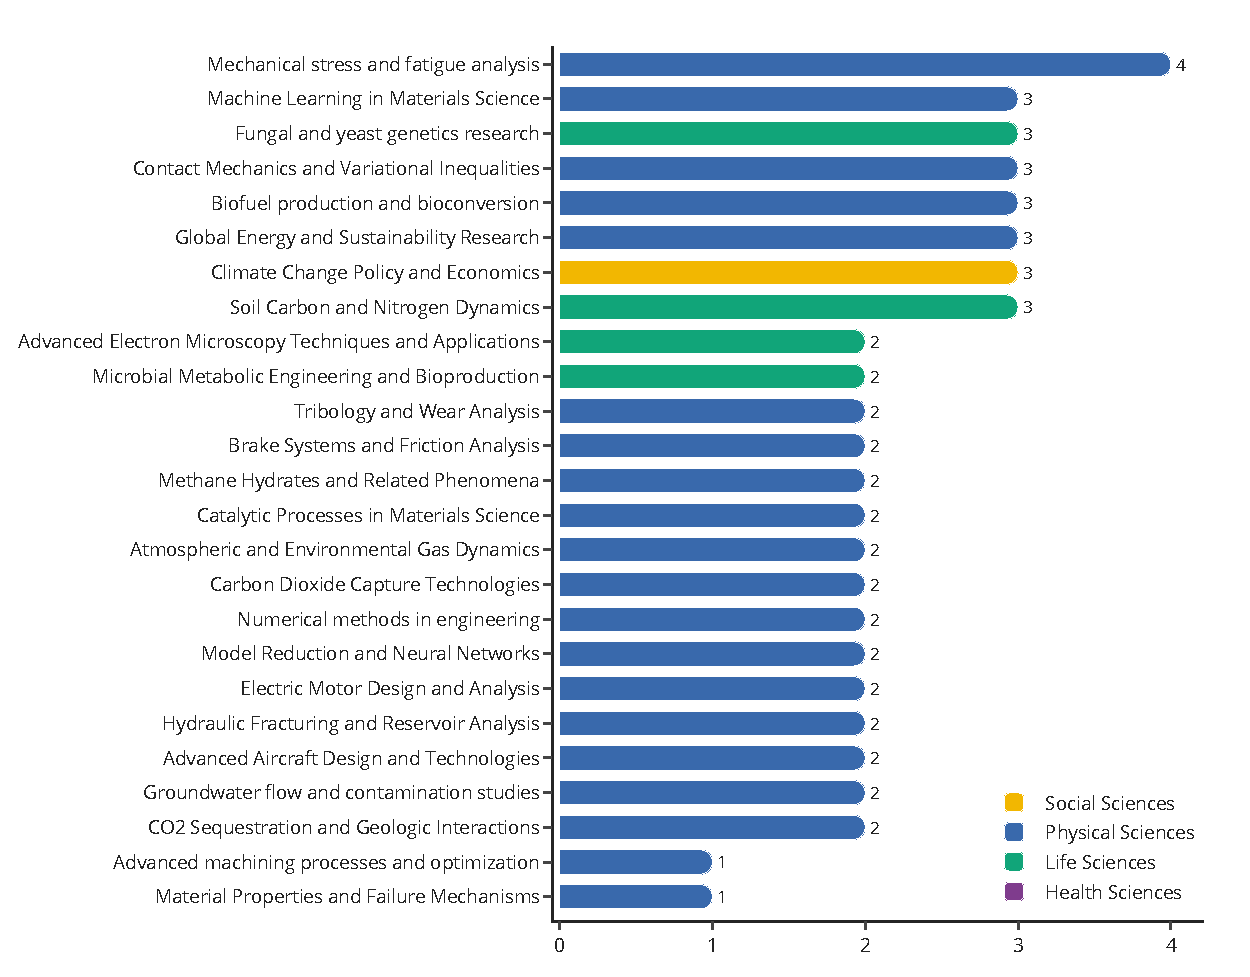
\includegraphics[width=\textwidth]{figures/topics_collaborations.pdf}
  \centering
  \caption{Principales thématiques de recherche identifiées dans les co-publications \entitiesacronym , pour la période \reportyear (OpenAlex)}
  \label{fig_topics_collaborations}
\end{figure}

{\footnotesize\topicscollaborationsinfo}


% Ecrire un commentaire sur les principales thématiques de recherches identifiées ci-dessous :





% Fin du commentaire sur les principales thématiques de recherches identifiées

\pagebreak

\section{Potentiel de collaboration identifié}

\begin{figure}[!h]
  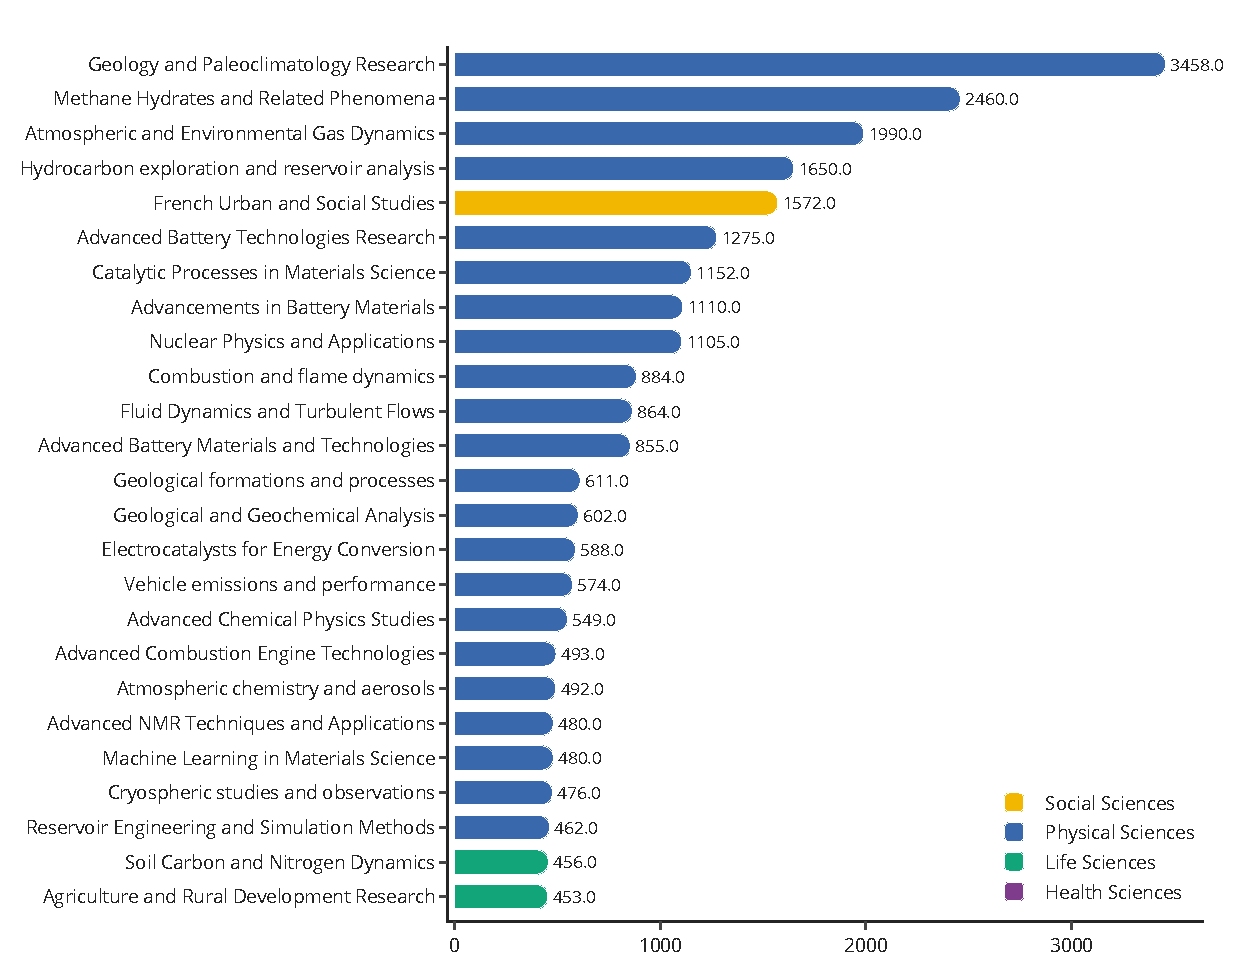
\includegraphics[width=\textwidth]{figures/topics_potential_collaborations.pdf}
  \centering
  \caption{Principales thématiques de recherche identifiées dans les publications \entitiesacronym (copublications exclues) pondérées par les thématiques des co-publications, pour la période \reportyear (OpenAlex)}
  \label{fig_topics_potential_collaborations}
\end{figure}

{\footnotesize\topicspotentialcollaborationsinfo}

Le potentiel de collaboration représente la capacité ou l'opportunité pour les deux institutions de travailler ensemble sur des sujets de recherche communs. Il est évalué en fonction de plusieurs facteurs :

\begin{itemize}
    \item - la fréquence des thématiques de recherche dans les travaux de chaque institution.
    \item - le taux de collaboration actuel : évalué à partir de l'importance actuelle de la collaboration des institutions sur ce sujet.
\end{itemize}

Un score de potentiel de collaboration élevé indique que le sujet est d'intérêt pour les deux institutions, mais qu'il y a encore une marge pour renforcer leur coopération. Cela permet d'identifier les domaines où des collaborations supplémentaires pourraient être particulièrement bénéfiques et stratégiques.

\bigskip


% Ecrire un commentaire sur les potentiel de collaboration identifié ci-dessous :





% Fin du commentaire sur les potentiel de collaboration identifié


\pagebreak

\section{Top 25 des structures internes avec le plus de co-publications}

\begin{figure}[!h]
  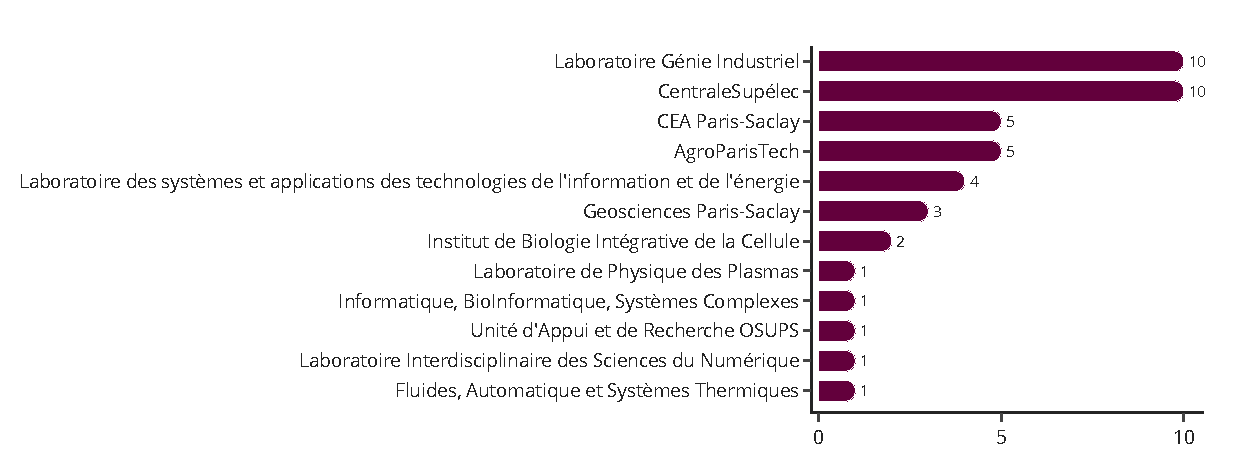
\includegraphics[width=\textwidth]{figures/institutions_lineage_collaborations.pdf}
  \centering
  \caption{Entités de la structure de référence avec le plus grand nombre de co-publications avec l'entité comparée, 2020-2025 (OpenAlex)}
  \label{fig_institutions_lineage_collaborations}
\end{figure}

{\footnotesize\institutionslineagecollaborationsinfo}

% Ecrire un commentaire sur le top 25 des structures internes avec le plus de co-publications ci-dessous :





% Fin du commentaire sur le top 25 des structures internes avec le plus de co-publications

\pagebreak

\section{Top 25 des co-publications par nombre de citations normalisées}

\begin{figure}[!h]
  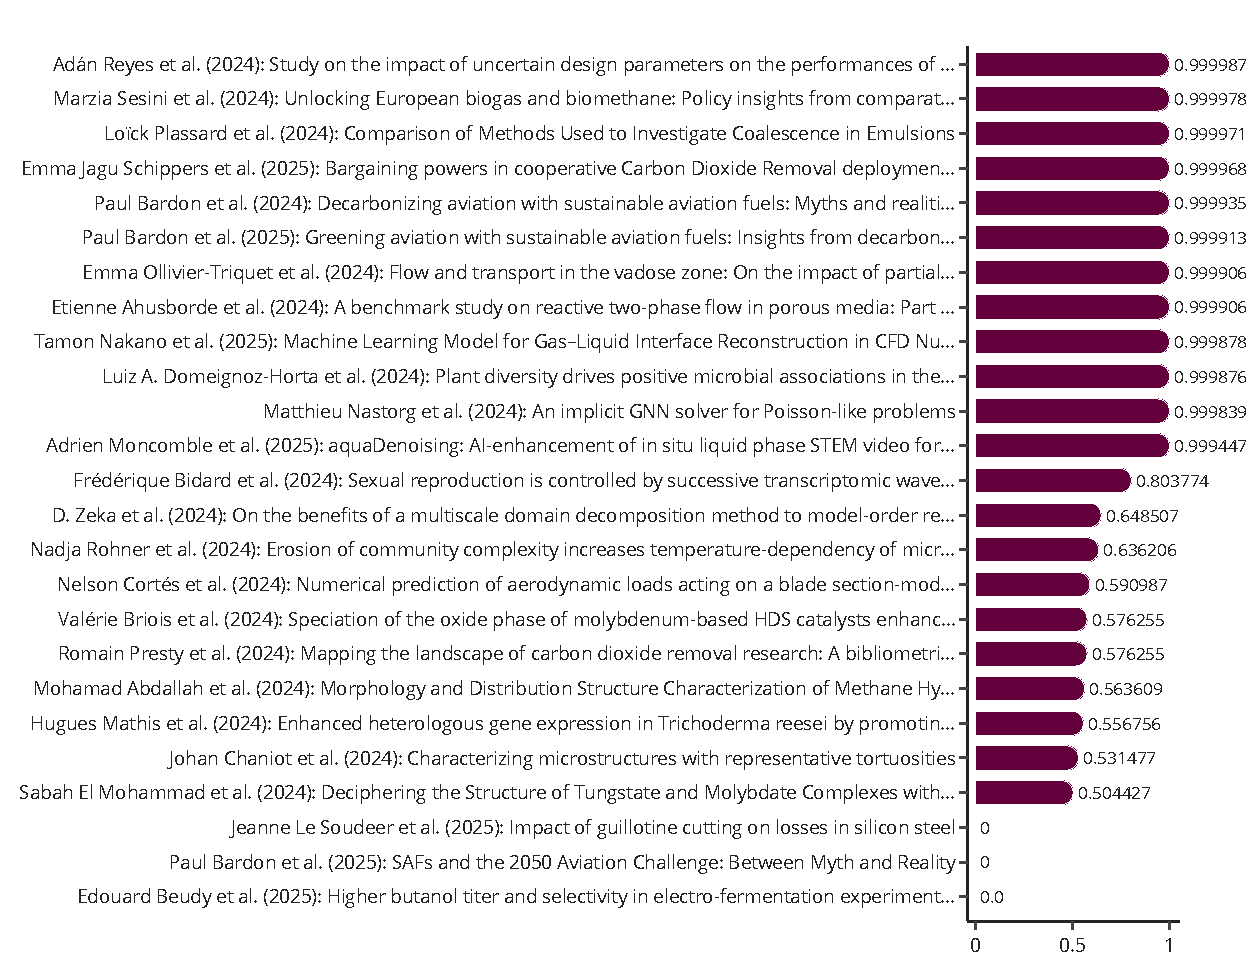
\includegraphics[width=\textwidth]{figures/works_collaborations_citationsnormalized.pdf}
  \caption{Co-publications entre \entitiesacronym sur la période \reportyear, ordonnées par à une métrique de citation normalisée (OpenAlex)}
  \label{fig_works_collaborations_citationsnormalized}
\end{figure}

{\footnotesize\workscollaborationscitationsnormalizedinfo}

Cette métrique évalue la performance relative des citations de chaque publication par rapport à l'ensemble des autres travaux du même domaine, sur la même année. Cette approche permet de traiter de manière normalisée l'influence et l'impact de chaque publication. Pour plus de détails, voir la documentation d'OpenAlex : \url{https://docs.openalex.org/api-entities/works/work-object#citation_normalized_percentile}

\bigskip

% Ecrire un commentaire sur le top 25 des co-publications par nombre de citations normalisées ci-dessous :





% Fin du  commentaire sur le top 25 des co-publications par nombre de citations normalisées


\pagebreak

\section{Top 25 des co-publications par nombre de citations}

\begin{figure}[!h]
  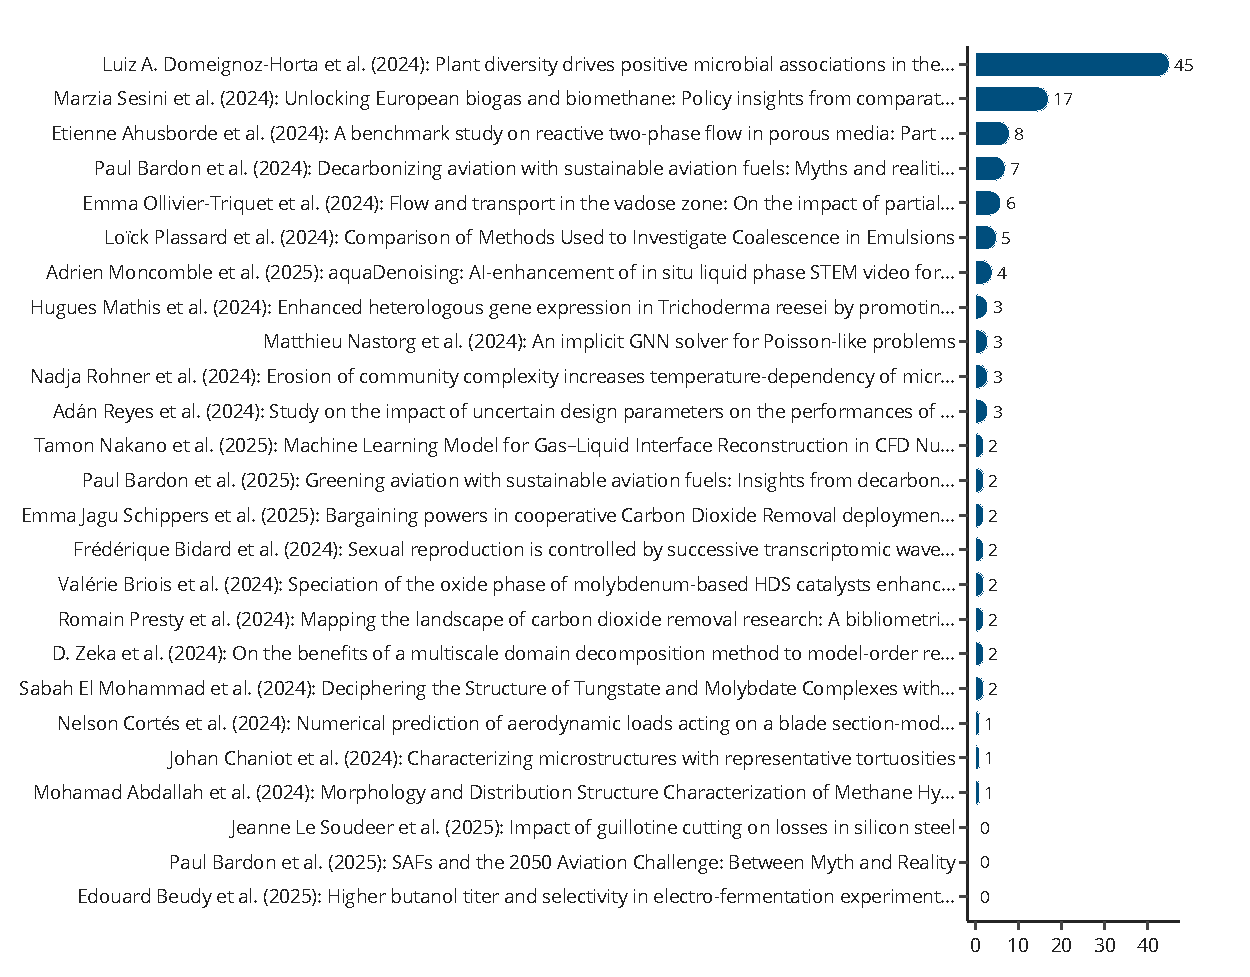
\includegraphics[width=\textwidth]{figures/works_collaborations_citationscount.pdf}
  \caption{Co-publications entre \entitiesacronym sur la période \reportyear, ordonnées par le nombre de citations (OpenAlex)}
  \label{fig_works_collaborations_citationscount}
\end{figure}

{\footnotesize\workscollaborationscitationscountinfo}




\makelastpagereport
 
\end{document}
